%-----------------------------------LICENSE------------------------------------%
%   This file is part of Mathematics-and-Physics.                              %
%                                                                              %
%   Mathematics-and-Physics is free software: you can redistribute it and/or   %
%   modify it under the terms of the GNU General Public License as             %
%   published by the Free Software Foundation, either version 3 of the         %
%   License, or (at your option) any later version.                            %
%                                                                              %
%   Mathematics-and-Physics is distributed in the hope that it will be useful, %
%   but WITHOUT ANY WARRANTY; without even the implied warranty of             %
%   MERCHANTABILITY or FITNESS FOR A PARTICULAR PURPOSE.  See the              %
%   GNU General Public License for more details.                               %
%                                                                              %
%   You should have received a copy of the GNU General Public License along    %
%   with Mathematics-and-Physics.  If not, see <https://www.gnu.org/licenses/>.%
%----------------------------------Preamble------------------------------------%
\documentclass{book}
\usepackage{graphicx}   % Needed for figures.
\usepackage{amsmath}    % Needed for align.
\usepackage{amssymb}    % Needed for mathbb.
\usepackage{amsthm}     % For the theorem environment.
\usepackage[nottoc]{tocbibind} % Bibliography in toc.
\usepackage{hyperref}   % Hyperlinks for URLs and references.

% Setup parameters for hyperlinks.
\hypersetup{colorlinks = true, linkcolor = blue}

%------------------------Theorem Styles-------------------------%
\theoremstyle{plain}
\newtheorem{theorem}{Theorem}[section]

% Define theorem style for default spacing and normal font.
\newtheoremstyle{normal}
    {\topsep}               % Amount of space above the theorem.
    {\topsep}               % Amount of space below the theorem.
    {}                      % Font used for body of theorem.
    {}                      % Measure of space to indent.
    {\bfseries}             % Font of the header of the theorem.
    {}                      % Punctuation between head and body.
    {.5em}                  % Space after theorem head.
    {}

% Define default environments.
\theoremstyle{normal}
\newtheorem{examplex}{Example}[section]
\newtheorem{definitionx}{Definition}[section]
\newtheorem{notationx}{Notation}[section]
\newtheorem{conjecture}{Conjecture}[section]
\newtheorem{question}{Question}[section]

\newenvironment{example}{%
    \pushQED{\qed}\renewcommand{\qedsymbol}{$\blacksquare$}\examplex%
}{%
    \popQED\endexamplex%
}

\newenvironment{definition}{%
    \pushQED{\qed}\renewcommand{\qedsymbol}{$\blacksquare$}\definitionx%
}{%
    \popQED\enddefinitionx%
}

\newenvironment{notation}{%
    \pushQED{\qed}\renewcommand{\qedsymbol}{$\blacksquare$}\notationx%
}{%
    \popQED\endnotationx%
}

\title{Khovanov Homology and Legendrian Simple Knots}
\author{Ryan Maguire}
\date{\today}

% No indent and no paragraph skip.
\setlength{\parindent}{0em}
\setlength{\parskip}{0em}

\graphicspath{{images/}}

\begin{document}
    \pagenumbering{gobble}
    \begin{titlepage}
        \centering
        \LARGE{\bfseries{Khovanov Homology and Legendrian Simple Knots}}
        \par\vspace{3.5cm}
        \par\vspace{4cm}
        \Large{\itshape{Ryan Maguire}}
        \par\vspace{1.5ex}
        \normalsize{\today}
    \end{titlepage}
    \nopagecolor
    \pagenumbering{roman}
    \tableofcontents
    \listoffigures
    \listoftables
    \clearpage
    \chapter*{Preface}
        \addcontentsline{toc}{chapter}{Preface}
    \clearpage
    \chapter*{Acknowledgements}
        \addcontentsline{toc}{chapter}{Acknowledgements}
    \clearpage
    \pagenumbering{arabic}
    \chapter{Knots and Links}
        %-----------------------------------LICENSE------------------------------------%
%   This file is part of Mathematics-and-Physics.                              %
%                                                                              %
%   Mathematics-and-Physics is free software: you can redistribute it and/or   %
%   modify it under the terms of the GNU General Public License as             %
%   published by the Free Software Foundation, either version 3 of the         %
%   License, or (at your option) any later version.                            %
%                                                                              %
%   Mathematics-and-Physics is distributed in the hope that it will be useful, %
%   but WITHOUT ANY WARRANTY; without even the implied warranty of             %
%   MERCHANTABILITY or FITNESS FOR A PARTICULAR PURPOSE.  See the              %
%   GNU General Public License for more details.                               %
%                                                                              %
%   You should have received a copy of the GNU General Public License along    %
%   with Mathematics-and-Physics.  If not, see <https://www.gnu.org/licenses/>.%
%----------------------------------Preamble------------------------------------%
\begin{figure}
    \centering
    \resizebox{\textwidth}{!}{%
        \includegraphics{endless_knot_celtic_style.pdf}
    }
    \caption{The Endless Knot}
    \label{fig:endless_knot_celtic_style}
\end{figure}
\begin{figure}
    \centering
    \resizebox{\textwidth}{!}{%
        \includegraphics{basket_weave_knot_celtic_style.pdf}
    }
    \caption{The Basket Weave Knot}
    \label{fig:basket_weave_knot_celtic_style}
\end{figure}
\begin{figure}
    \centering
    \resizebox{!}{0.4\textheight}{%
        \includegraphics{borromean_rings_tricursal_valknut.pdf}
    }
    \caption{The Tricursal Valknut}
    \label{fig:borromean_rings_tricursal_valknut}
\end{figure}
Knots have long been marveled as a source of art and beauty. In the Book of
Kells, a Celtic work containing the four gospels of the New Testament created
sometime between the the $7^{\small\textrm{th}}$ and $9^{\small\textrm{th}}$
centuries \cite[p.~108]{Nordenfalk1977}, intricate drawings of complicated
knots and links are found. Many pages contained depictions of the endless knot
(Fig.~\ref{fig:endless_knot_celtic_style}) and the basket weave knot
(Fig.~\ref{fig:basket_weave_knot_celtic_style}). The endless knot also appears
in Tibetan Buddhism, being one of the ``eight auspicious symbols''
\cite[p.~11]{BeerTibetanSymbols}. The Borromean rings
(Fig.~\ref{fig:borromean_rings_no_shadow}) appear in Celtic, Tibetan,
and Viking cultures
\cite[p.~129]{VikingWomenJesch}%
\footnote{%
    The Legend of Hildr is depicted on the stone carving in this
    reference. The tricursal \textit{Valknut}
    (Fig.~\ref{fig:borromean_rings_tricursal_valknut}),
    the Viking-Germanic version of Borromean rings,
    can be seen on the third carving from the top.
},
and the trefoil (Fig.~\ref{fig:trefoil_knot})
appears in Celtic, Islamic, Norse, and Tibetan art as well.
\par\hfill\par
As a mathematical discipline, the origins of knot theory
date back to the $18^{\small\textrm{th}}$ and
$19^{\small\textrm{th}}$ centuries with semi-rigorous treaties of
the subject being formed by Vandermonde in 1771 \cite{Vanermonde1771}
and Gauss in 1833 \cite[p.~1327]{RiccaNipotaGaussLinkingNumber}.
Serious investigations into the field are often first attributed to Peter Tait
who established some of the earliest tabulations of knots and put forward
several conjectures in a treatise published in 1885. Tait's motivation was
primarily the conjecture of Lord Kelvin who believed that chemical properties
of matter could be explained by atoms being \textit{knotted}, in some sense.
J.J. Thompson expanded this idea and developed some of the earlier mathematical
properties of knots, only to abandon the hypothesis altogether with his
discovery of the electron. An so vortex theory died, but knot theory lives on.
\begin{figure}
    \centering
    \resizebox{!}{0.4\textheight}{%
        \includegraphics{borromean_rings_no_shadow.png}
    }
    \caption{The Borromean Rings}
    \label{fig:borromean_rings_no_shadow}
\end{figure}

        \section{Basic Definitions and Invariants}
    Following \cite[p.~15]{LivingstonKnotTheory}, we define a knot as follows.
    \begin{definition}[\textbf{Knot}]
        A knot is a polygonal (piece-wise linear) embedding
        $\gamma:\mathbb{S}^{1}\rightarrow\mathbb{R}^{3}$ of the circle into
        three dimensional Euclidean space.
    \end{definition}
    While it is possible to define knots using \textit{continuous} embeddings,
    such a definition provides for the existence of
    \textit{wild knots} \cite{FoxArtinWildKnots1948}.\footnote{%
        See \cite{BrowneWildKnots} for how to procedurally generate wild knots.
    }
    \textit{Smooth} embeddings can similarly be used, albeit at the expense of
    a slightly harder definition of \textit{knot equivalence}. In the
    polygonal case this comes with ease. Given a piece-wise linear embedding
    $\gamma:\mathbb{S}^{1}\rightarrow\mathbb{R}^{3}$ with vertices
    $P_{1},\,\dots,\,P_{n}$ we are allowed to deform $\gamma$ into a new one
    $\gamma'$ formed by the (ordered) vertices $P_{1},\,\dots,\,P_{n},\,P'$
    such that the triangle $\Delta{P}_{n}P'P_{1}$ only intersects $\gamma$
    along the line segment $\overline{P_{1}P_{n}}$. This is called an
    \textit{elementary knot equivalence}. With this we define equivalent knots.
    \begin{definition}[\textbf{Equivalent Knots}]
        Equivalent knots are polygonal embeddings
        $\gamma,\gamma':\mathbb{S}^{1}\rightarrow\mathbb{R}^{3}$ and
        that differ by
        a finite number of elementary knot equivalences.
    \end{definition}
    

        %-----------------------------------LICENSE------------------------------------%
%   This file is part of Mathematics-and-Physics.                              %
%                                                                              %
%   Mathematics-and-Physics is free software: you can redistribute it and/or   %
%   modify it under the terms of the GNU General Public License as             %
%   published by the Free Software Foundation, either version 3 of the         %
%   License, or (at your option) any later version.                            %
%                                                                              %
%   Mathematics-and-Physics is distributed in the hope that it will be useful, %
%   but WITHOUT ANY WARRANTY; without even the implied warranty of             %
%   MERCHANTABILITY or FITNESS FOR A PARTICULAR PURPOSE.  See the              %
%   GNU General Public License for more details.                               %
%                                                                              %
%   You should have received a copy of the GNU General Public License along    %
%   with Mathematics-and-Physics.  If not, see <https://www.gnu.org/licenses/>.%
%----------------------------------Preamble------------------------------------%
\section{Representing Knots}
    Now that we have the basic definitions we move on to the problem of
    describing knots with finite data. An explicit parametrization
    $\gamma:\mathbb{S}^{1}\rightarrow\mathbb{R}^{3}$ could be given, but this
    is rarely done in practice and for good reason. As the number of crossings
    in a knot diagram increases it becomes harder to describe smooth embeddings
    via elementary functions.\footnote{%
        Certain families of knots, like the torus knots, are
        exceptions to this rule. Smooth embeddings can be given explicitly via
        trigonometric functions.
    }
    Polygonal embeddings can be described by specifying the vertices, but this
    becomes an exercise in tedium as the number of crossings increases.
    Instead we use one of several (similar but different) methods to describe
    the crossings of a knot diagram and encode their positions relative to
    each other. Certain algorithms will develop more naturally via the use
    of one representation over the other, and so the entirety of this section
    is devoted to describing these methods in detail.
    \subsection{Gauss Codes}
        \begin{figure}
            \centering
            \resizebox{0.5\textwidth}{!}{%
                \includegraphics{%
                    trefoil_knot_oriented_with_gauss_code.pdf
                }
            }
            \caption{Gauss Code for the Right-Handed Trefoil}
            \label{fig:right_handed_trefoil_gauss_code}
        \end{figure}
        Given an \textit{oriented} knot diagram $K$ with $N$ crossings, we
        label the crossings $0$ to $N-1$. Any ordering will suffice, but
        usually one picks a point and then travels along the knot, following
        the orientation, and labels the crossings in increasing order as they
        pass. Now pick a starting point and following along the knot. As you
        come upon a crossing write down its number and whether you are on the
        over strand or the under strand. Do this until you return to your
        starting point. Each crossing will occur twice in your list, once as an
        over crossing and once as an under crossing, so at the end you will
        have a sequence with $2N$ entries. This is called the
        \textbf{unsigned Gauss code} of the knot. It is dependent on the
        knot diagram, your choice of labeling, the orientation given, and your
        choice in starting point. Consider
        Fig.~\ref{fig:right_handed_trefoil_gauss_code}. With this particular
        labeling, orientation, and starting point we obtain
        \texttt{O0 U1 O2 U0 O1 U2}. If we consider the left-handed trefoil with
        a similar labeling scheme, but choose a different starting point, we
        obtain the same string (Fig.~\ref{fig:left_handed_trefoil_gauss_code}).
        The right-handed and left-handed trefoils are
        not equivalent \cite[p.~200-204]{DehnGroupTheoryAndTopology} and so
        this description does not uniquely capture the knot diagram.\footnote{%
            It is not all bad, however. There exists an algorithm to
            convert unsigned Gauss code into Dowker-Thistlethwaite code
            \cite{KatlasDTCode}, and vice-versa. In \cite{DOWKER198319} it is
            proved that two \textit{prime} knots with the same
            Dowker-Thistlethwaite code are either equivalent or are mirror
            reflections of one another. Hence unsigned Gauss code
            \textit{almost} distinguishes prime knots.
        }
        \begin{figure}
            \centering
            \resizebox{0.5\textwidth}{!}{%
                \includegraphics{%
                    trefoil_knot_mirror_oriented_with_gauss_code.pdf
                }
            }
            \caption{Gauss Code for the Left-Handed Trefoil}
            \label{fig:left_handed_trefoil_gauss_code}
        \end{figure}
        \par\hfill\par
        We modify Gauss code slightly in order to obtain
        \textbf{extended Gauss code}, also called \textbf{signed Gauss code}.
        We perform the same steps as before, but now we also write down the
        \textit{sign} of each crossing as we pass. A minor change, but one
        that is powerful enough to detect knots.
        \begin{theorem}
            If two knots have the same extended Gauss code, then they are
            equivalent.
        \end{theorem}
        \begin{proof}
            There exists an algorithm to explicitly construct the knot diagram
            of a knot from extended Gauss code. See
            \cite{KauffmanVirtualKnots1999}.
        \end{proof}
        \begin{figure}
            \centering
            \resizebox{0.5\textwidth}{!}{%
                \includegraphics{%
                    trefoil_knot_oriented_with_extended_gauss_code.pdf
                }
            }
            \caption{Extended Gauss Code for the Right-Handed Trefoil}
            \label{fig:trefoil_knot_oriented_with_extended_gauss_code}
        \end{figure}
        \begin{figure}
            \centering
            \resizebox{0.5\textwidth}{!}{%
                \includegraphics{%
                    trefoil_knot_mirror_oriented_with_extended_gauss_code.pdf
                }
            }
            \caption{Extended Gauss Code for the Left-Handed Trefoil}
            \label{fig:trefoil_knot_mirror_oriented_with_extended_gauss_code}
        \end{figure}
        The extended Gauss code for the right-handed trefoil knot is shown in
        Fig.~\ref{fig:trefoil_knot_oriented_with_extended_gauss_code}.
        Contrasting this with the left-handed trefoil in
        Fig.~\ref{fig:trefoil_knot_mirror_oriented_with_extended_gauss_code}
        shows we have successfully differentiated between the two. The
        guarantee of this success can by examining how Gauss codes change
        under mirror reflection. Appealing to
        Fig.~\ref{fig:crossing_signs} we see that positive and negative
        crossings will swap. Moreover, the type of the crossings will swap
        (over to under, and vice-versa). For the unsigned Gauss code of the
        right-handed trefoil (Fig.~\ref{fig:right_handed_trefoil_gauss_code})
        reflecting \texttt{O0 U1 O2 U0 O1 U2} yields
        \texttt{U0 O1 U2 O0 U1 O2}. By shifting the sequence, which amounts
        to picking a new starting point, we see that this can become
        \texttt{O0 U1 O2 U0 O1 U2} once again, yielding our original problem.
        Introducing signs we see that the right-handed trefoil has all
        positive crossings. Reflecting this will yield all negative crossings,
        meaning the extended Gauss codes will differ, in precise agreement
        with our two figures.
        \par\hfill\par
        The three Reidemeister moves translate to operations on Gauss code.
        A loop in a knot diagram means the crossing will be seen successively
        in the code. Type I means we may delete such a loop, which translates
        to removing the entries in the Gauss code.
        \par\hfill\par
        Type II tells us to look for pairs of numbers $m,\,n$ where we see
        \texttt{Om On} followed by \texttt{Um Un} somewhere else in the code.
        Conversely we may look for \texttt{Um Un} followed by \texttt{Om On}
        later on. Additionally, the ordering is allowed to switch and we may
        seek \texttt{Om On} followed by \texttt{Un Um}, or
        \texttt{Um Un} followed by \texttt{On Om}. Type II tells us should we
        find such a pair of integers, we may delete the four entries from the
        code.
        \par\hfill\par
        Unsurprisingly, Type III is the hardest to translate to operations on
        Gauss code. Here we seek triples of numbers
        $\ell,\,m,\,n$ with \texttt{Um Un}, \texttt{Om Ol},
        and \texttt{On Ul} in the code. We may also swap all of the crossing
        types, interchanging \texttt{O} with \texttt{U} and vice-versa.
        We keep \texttt{Um Un} fixed but swap the order of the other two.
        That is, \texttt{Om Ol} becomes \texttt{Ol Om} and
        \texttt{On Ul} becomes \texttt{Ul On}. There is no reduction in the
        length of the Gauss code here, just as Type III does not reduce the
        number of crossings in the diagram.
        \par\hfill\par
        From a technical perspective an extended Gauss code is a string of
        ordered triples. The length of the string is $2N$ for some integer
        $N\in\mathbb{N}$ and the sequence must satisfy the following
        conditions.
        \begin{enumerate}
            \item
                The ordered triples are of the form $(n,\,t,\,s)$ with
                $n\in\mathbb{Z}_{N}$, $t\in\{\,O,\,U\,\}$, and
                $s\in\{\,-1,\,1\,\}$. $n$ is the \textit{index}, $t$ is the
                \textit{type}, and $s$ is the \textit{sign}.
            \item
                Every $n\in\mathbb{Z}_{n}$ occurs in exactly two of the
                triples in the sequence, once with $t=O$ and once with
                $t=U$.
            \item
                The sign $s$ does not change between tuples with the same
                index.
        \end{enumerate}
        \begin{figure}
            \centering
            \includegraphics{chain_link_fence_knot_virtual.pdf}
            \caption{Chain Link Fence Virtual Knot Diagram}
            \label{fig:chain_link_fence_knot_virtual}
        \end{figure}
        Hence \texttt{O0+ O1+ O0- U1+} is invalid for two reasons. For one
        the sign changes for \texttt{0}, and secondly \texttt{U0} never occurs.
        Correcting this we see that \texttt{O0+ U1+ U0+ O1+} satisfies all of
        the constraints. If we try do draw a knot diagram that admits this
        extended Gauss code we come to the awkward situation of being forced
        to introduce a third crossing. We circle this \textit{virtual} crossing
        and obtain Fig.~\ref{fig:chain_link_fence_knot_virtual}.\footnote{%
            It is easy to be mislead here and believe
            \texttt{O0+ U1+ U0+ O1+} should create a two crossing unknot
            obtained by performing a Type II move on the unit circle. This will
            instead create \texttt{O0+ U0+ U1- O1-}.
        }
        For reasons that will become apparent in the following pages, we shall
        call this the \textbf{chain-link fence knot}. Appealing to graph
        theory, we know it is impossible to draw the complete graph
        $K_{5}$ in the plane without introducing crossings. By introducing a
        handle into the plane we can get a bonafide embedding of
        $K_{5}$ onto a torus. Similarly for any graph (like
        Fig.~\ref{fig:graph_has_genus_001}) we can draw it in the
        plane and then introduce handles at all of the \textit{virtual}
        crossings to get ride of them and obtain an embedding of the graph
        into a higher genus surface (Fig.~\ref{fig:graph_has_genus_002}).
        \begin{figure}
            \centering
            \begin{minipage}[b]{0.49\textwidth}
                \centering
                \resizebox{\textwidth}{!}{%
                    \includegraphics{graph_has_genus_001.pdf}
                }
                \caption{Non-Embedded Graph}
                \label{fig:graph_has_genus_001}
            \end{minipage}
            \hfill
            \begin{minipage}[b]{0.49\textwidth}
                \centering
                \resizebox{\textwidth}{!}{%
                    \includegraphics{graph_has_genus_002.pdf}
                }
                \caption{Embedded Graph}
                \label{fig:graph_has_genus_002}
            \end{minipage}
        \end{figure}
        \par\hfill\par
        We conduct a complete mimicry of this graph-theoretic idea for
        extended Gauss codes. The chain-link fence knot requires one
        virtual crossing allowing us to embed it onto the torus
        (Fig.~\ref{fig:chain_link_fence_knot_on_torus}). The resulting object
        is called a \textbf{virtual knot}. There are at least three equivalent
        means of thinking about virtual knots. First is as valid Gauss codes
        up to \textbf{virtual knot equivalence}, a translation of the
        Reidemeister for arbitrary extended Gauss codes. Secondly we may think
        of them as smooth or polygonal embeddings of $\mathbb{S}^{1}$ into
        $M\times\mathbb{R}$ where $M$ is a compact orientable surface.
        Equivalence is then given by \textit{stabilization}
        (See \cite{CarterKamadaSaitoVirtualKnotCobordisms}). We may also think
        of virtual knots as smooth or polygonal embeddings into
        $M\times\mathbb{R}$ for some compact orientable surface $M$ where $M$
        is of \textit{minimal genus} \cite{KuperbergVirtualLink}.
        With this definition, classical knots (those without virtual crossings)
        are precisely the virtual knots with $M=\mathbb{S}^{2}$,
        the unit sphere.
        \begin{figure}
            \centering
            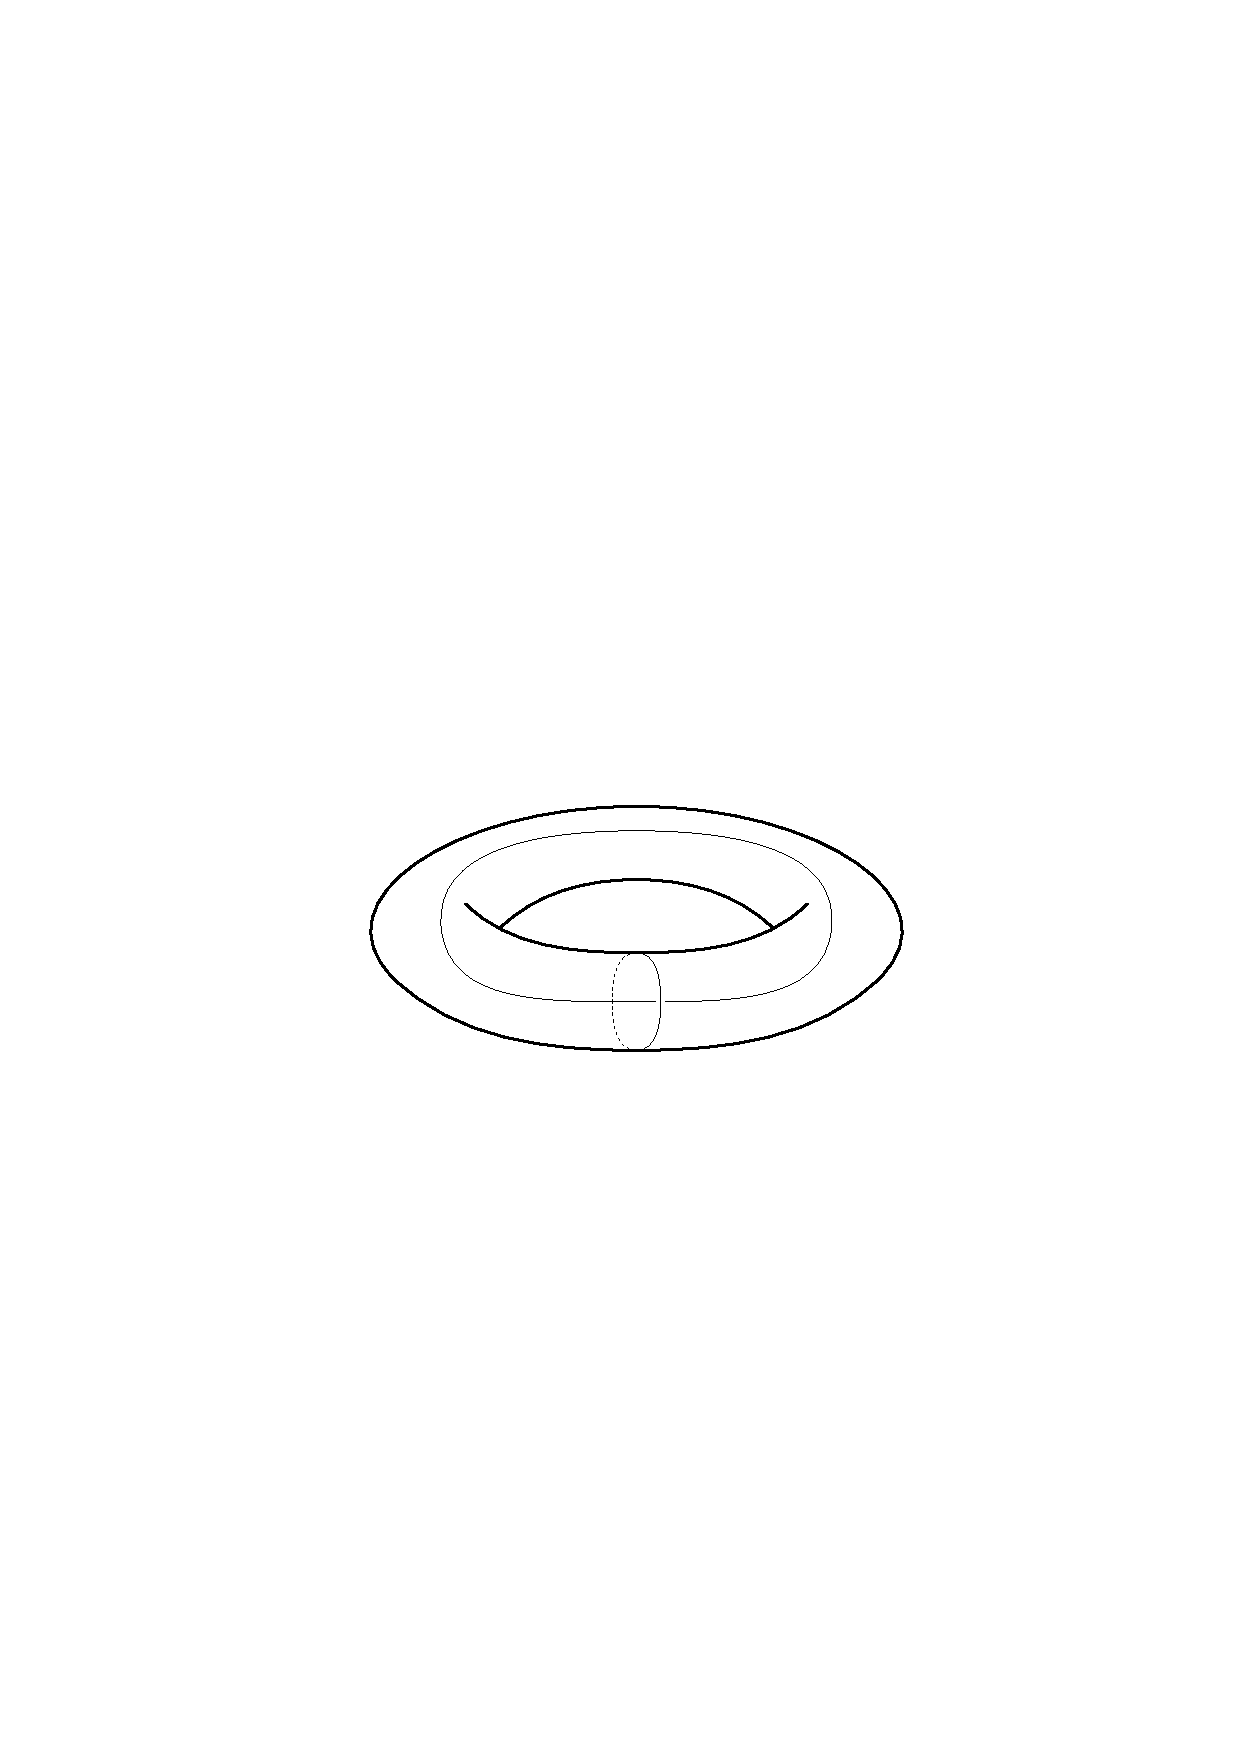
\includegraphics{chain_link_fence_knot_on_torus.pdf}
            \caption{Chain Link Fence Knot on a Torus}
            \label{fig:chain_link_fence_knot_on_torus}
        \end{figure}
        \par\hfill\par
        This last definition borrows the same difficulty from graph theory.
        While attaching handles at all of the $g$ virtual crossings yields an
        embedding into $M\times\mathbb{R}$ where $M$ is the compact orientable
        surface of genus $g$, it may have been possible to use fewer handles.
        Consider again Figs.~\ref{fig:graph_has_genus_001} and
        \ref{fig:graph_has_genus_002} where we created an embedding into the
        genus 3 compact surface. The starting graph was actually planar and
        need no additional handles (Fig.~\ref{fig:graph_has_genus_003}).
        \begin{figure}
            \centering
            \resizebox{0.5\textwidth}{!}{%
                \includegraphics{graph_has_genus_003.pdf}
            }
            \caption{Planar Embedding}
            \label{fig:graph_has_genus_003}
        \end{figure}
        \par\hfill\par
        While it is possible to compute the minimal genus of a virtual knot,
        we will not need such an algorithm. Our later work will be motivated
        by a more classical problem which is related to this difficulty.
        If one is given an extended Gauss code (a \textit{virtual knot}),
        is it possible to determine if there is a (classical) knot diagram
        that realizes this code? We can indeed do this in linear time.
        \par\hfill\par
        A valid Gauss code with $2N$ entries describes a virtual knot with
        $N$ crossings. Suppose we have embedded our virtual knot into
        $M\times\mathbb{R}$ where $M$ is a compact orientable surface of
        minimal genus. Projecting down the $\mathbb{R}$ component we obtain
        a graph embedded into $M$ where the crossings form the vertices. The
        graph is 4-valent, so by the hand-shaking theorem there are
        $2N$ edges. We are in effect decomposing $M$ into a CW complex with
        $N$ 0-cells, $2N$ 1-cells, and $F$ 2-cells. If we can compute $F$ we
        will obtain $g$ via Euler's formula:
        \begin{equation}
            V-E+F=2-2g
        \end{equation}
        Substituting $V=N$ and $E=2N$ we have:
        \begin{equation}
            g=\frac{2+N-F}{2}
        \end{equation}
        If we can compute $F$ we will have also computed $g$, and if
        $g\ne{0}$ we will know the extended Gauss code does not describe the
        knot diagram of a classical knot. We now describe how to compute $F$.
        \par\hfill\par
        \begin{figure}
            \centering
            \includegraphics{thickened_crossings.pdf}
            \caption{Signed Thickened Crossings}
            \label{fig:thickened_crossings}
        \end{figure}
        Thicken the knot projection so that the crossings look like
        Fig.~\ref{fig:thickened_crossings}. Begin traveling along the thickened
        knot, following the orientation given by the Gauss code, and place your
        finger on the left wall at all times. When you come to a crossing,
        turn left so that your finger remains continuously on the wall of the
        thickened knot. Continue doing this until you return to your starting
        point. You will have just traced out a $k$-gon for some
        $k\in\mathbb{N}$. Attach a 2-cell by gluing along this polygon.
        Continue doing this until all $4N$ of the corners of the thickened
        crossings (again, appeal to Fig.~\ref{fig:thickened_crossings}) have
        be traveled. The total number of faces, which is the total number of
        cycles you've traveled, has now been computed. We require $4N$ steps,
        and so our algorithm does indeed run in linear time.
        \par\hfill\par
        The steps described translate to jumping between the entries in the
        Gauss code in a well-defined manner. \textit{Going left} means changing
        crossing type and then walking with or against the orientation.
        That is, if you come to entry \texttt{Ons}, with \texttt{n} the index
        and \texttt{s} the sign, jump ahead to \texttt{Uns}, changing crossing
        type. You then proceed to either the next entry in the Gauss code or
        the previous entry depending on the value of the sign \texttt{s}.
        This amounts to walking forwards or backwards. The correct direction
        can be computed from Fig.~\ref{fig:thickened_crossings}. If you are at
        the final entry and need to proceed forward, loop back around to the
        start. Similarly, if you are at the starting entry and need to move
        backwards, jump ahead to the end of the Gauss code. By repeatedly
        doing this we can compute the number of cycles and consequently
        calculate the genus.
        \par\hfill\par
        Applying this algorithm to the standard 3-crossing trefoil (either the
        left handed or right handed) will yield 5 faces, giving us a genus of
        0. The chain link fence knot \texttt{O0+ U1+ U0+ O1+} produces 2 faces,
        and so we end up with a genus 1 knot diagram which can be embedded on
        the torus. The faces, and the reason for the name
        \textit{chain link fence}, can be easily seen if we conduct our drawings
        on the flat torus (Fig.~\ref{fig:chain_link_fence_knot_on_flat_torus}).
        If we lift to the universal cover of the torus, which is the Euclidean
        plane, we can see the two aforementioned faces, as well as a chain
        link fence pattern
        (Fig.~\ref{fig:chain_link_fence_knot_on_flat_torus_universal_cover}).
        \begin{figure}
            \centering
            \includegraphics{chain_link_fence_knot_on_flat_torus.pdf}
            \caption{Chain Link Fence Virtual Knot on a Flat Torus}
            \label{fig:chain_link_fence_knot_on_flat_torus}
        \end{figure}
        \begin{figure}
            \centering
            \resizebox{\textwidth}{!}{%
                \includegraphics{%
                    chain_link_fence_knot_on_flat_torus_universal_cover.pdf
                }
            }
            \caption{Lift of the Chain Link Fence to the Universal Cover}
            \label{fig:chain_link_fence_knot_on_flat_torus_universal_cover}
        \end{figure}
        \par\hfill\par
        It should be considered a pleasant bonus if a knot invariant is also
        an invariant for virtual knots. It is especially enjoyable when an
        algorithm for a knot invariant can be copied for virtual knots with
        little or no additional effort. But, before proceeding, two warnings
        are worth mentioning.
        \par\hfill\par
        The operations of the Reidemeister moves are stricter for virtual knots
        via extended Gauss code. For classical knots, should we find
        \texttt{On Om} followed by \texttt{Un Um}, or any re-ordering thereof,
        we can apply Type II and delete the four entries from the code. This is
        not so for virtual knots. Indeed, were it true the chain link fence
        would be equivalent to the unknot. The sign is crucial for a correct
        description of Type II moves in the virtual setting. For a true
        Type II move, the signs alternate. This in agreement with the fact that
        Type II does not change the writhe of a diagram. So, should we find
        \texttt{On+ Om-} followed by \texttt{Un+ Um-}, or any re-ordering
        thereof, we may apply Type II and delete the four entries, be it a
        classical or virtual knot.
        \par\hfill\par
        Lastly, the algorithm described previously computed the genus of a
        virtual knot \textit{diagram}, and not the minimal genus of all
        possible equivalent diagram. By application of Type II it is possible
        give the right-handed trefoil a genus 1 knot diagram, for example
        \texttt{O0+ U1+ O2+ O3- O4+ U0+ U3- U2+ O1+ U4+}. The Reidemeister
        moves may change the genus of a diagram.
    \subsection{Planar Diagrams}
        Planar diagram code, commonly called PD code, is one of the more popular
        representations found in programming libraries. We start with an
        oriented knot diagram and pick a starting point. We follow the
        orientation and label the \textit{arcs}, the edges between crossings,
        in increasing order from $0$ to $2N-1$ where $N$ is the number of
        crossings. Once the arcs have been labeled we once again walk around
        the knot diagram and each time we come across an under crossing we write
        down \texttt{X[a,b,c,d]} where \texttt{a} is the number of the arc you
        are coming from, \texttt{c} is the arc you'll be leaving through,
        \texttt{b} is the arc to your \textit{right}, and \texttt{d} is the
        arc to your \textit{left}. The PD code of the diagram is the ordered
        sequence of 4-tuples \texttt{X[a,b,c,d]} for each under crossing you
        encounter in the order you encounter them. Using
        Fig.~\ref{fig:trefoil_knot_arcs_labeled}, the right-handed trefoil can
        represented by writing \texttt{X[1,5,2,4],X[3,1,4,0],X[5,3,0,2]}.
        \begin{figure}
            \centering
            \includegraphics{trefoil_knot_arcs_labeled.pdf}
            \caption{Trefoil Knot with Arcs Labeled}
            \label{fig:trefoil_knot_arcs_labeled}
        \end{figure}
        \par\hfill\par
        Planar diagram code can recover unsigned Gauss code, but moreover
        the sign of the crossings can also be computed. Since the arcs are in
        increasing order, we have that for each entry
        \texttt{X[a,b,c,d]}, the difference $\texttt{c}-\texttt{a}$ is either
        1 or $1-N$, with $1-N$ occurring if and only of \texttt{a} is the final
        arc in the ordering. In contrast, the difference $\texttt{d}-\texttt{b}$
        can be $+1$ or $-1$, once reduced mod $N$. $+1$ means the crossing is
        positive and $-1$ means the crossing is negative. Whether this is a
        lucky coincidence, or if the signing of the crossings was originally
        chosen to yield this result, one must admit it is a rather elegant
        computation.
        \par\hfill\par
        Since the signs of the crossings can be computed, and since
        PD code can determine the unsigned Gauss code, we immediately see that
        PD code and extended Gauss code have the same information. Because of
        this one may use PD codes for virtual knots as well, but the phrasing
        \textit{virtual planar diagram code} is rather unfortunate for
        non-planar virtual knot diagrams. At any rate, it is \textit{not}
        common practice to use PD codes to represent virtual knots. Indeed,
        some programming libraries have checks to ensure the input PD code
        represents a planar knot diagram before allowing computations to be
        performed.
    \subsection{Dowker-Thistlethwaite Notation}
        Dowker-Thistlethwaite code (DT code for short) compactly describes
        knots. Because of this it is used in tabulation efforts where millions
        of distinct knot are listed in massive tables
        (see, for example \cite{Burton2020TheN3} and \cite{regina}).
        \par\hfill\par
        Start with an oriented knot diagram and choose a starting point.
        Walk along the knot, following the orientation, and number the
        crossings as you pass them in increasing order. For each odd number,
        if you are on the under strand as you pass the crossing,
        prepend a minus sign. Should you come upon a crossing you've already
        marked, label it again with the second number second number as well.
        At the end you should have a permutation of all numbers (with possible
        minus signs) between $0$ and $2N-1$ where $N$ is the number of
        crossings, each crossing having two numbers assigned to it. If the knot
        diagram is \textit{planar} and represents a classical knot, by a
        parity argument and the Jordan curve theorem we see that each crossing
        will have one odd number and one even number associated to it. Pair
        the numbers together into tuples $(2n,\,\pm{2m+1})$ corresponding to the
        same crossing. Lastly, order the tuples lexicographically by giving
        preference to the first entry (the even number in the tuple).
        The DT code is the corresponding ordered sequence of even numbers,
        with minus signs included.\footnote{%
            In computer science it is very common to start numbering at zero,
            which is what we have done several times throughout. In the
            original paper the labeling start at 1. Because of this the
            \textit{even} numbers are given plus and minus signs, and the
            tuples are ordered with respect to the \textit{odd} numbers. A
            minor change, but a very important one. Failure to be consistent
            can result in the wrong DT code!
        }
        \par\hfill\par
        Quite verbose, let us consider an example.
        Fig.~\ref{fig:trefoil_knot_oriented_001} depicts an oriented
        right-handed trefoil, let's start with this. Choosing the top-most
        point, we obtain the sequence of ordered tuples
        $(0,\,3)$, $(2,\,5)$, $(4,\,1)$. So our DT code for the right-handed
        trefoil is \texttt{3 5 1}. The same DT code is attainable for the
        left-handed trefoil, meaning the notation is mirror insensitive. Still,
        it is extremely compact. The following theorem further justifies its
        use.
        \begin{theorem}[Dowker, Thistlethwaite 1983]
            If two prime knots have the same DT code, then they are either
            equivalent or are mirrors of one another.
        \end{theorem}
        \begin{proof}
            See \cite{DOWKER198319}.
        \end{proof}
        Since knot tabulation rarely differentiates between mirrors, and
        almost exclusively concerns itself with the listing of prime knots,
        DT code is perfect for such an endeavor.
        \par\hfill\par
        Since the code consists entirely of odd numbers we can obtain the
        \textbf{simplified DT code} by subtracting one and dividing by two,
        doing this to each element. The trefoil then becomes
        \texttt{1 2 0}. Furthermore, should we be concerned with knots of
        no more than 26 crossings, we can substitute numbers with letters.
        This is the \textbf{alphabetical DT code}. The trefoil becomes
        \texttt{bca}. Should a minus sign be part of the original DT code
        we would add one and divide by two for the simplified code, and the
        alphabetical code would be given using a capital letter. For example,
        the knot $8_{19}$ in the Rolfsen table
        has the alphabetical DT code
        \texttt{bdFaGHCE}. In our presentation of knot tables we will
        exclusively use the alphabetical DT notation for its brevity.
    \subsection{Braids}
        Braids are one of the original means of representing knots
    \subsection{Tangles}
    \subsection{Tait Graphs}

        \section{Knot Recognition}
    Now that we have the means to represent knots, we take a brief moment to
    discuss \textit{recognizing} them. Knot theory is an extremely
    challenging field when it comes to numerical
    analysis. Many other tasks regularly enjoy polynomial time algorithms and
    highly optimized implementations. As a popular example, signal processing
    makes frequent use of the Fast Fourier Transform (FFT) which runs in
    $O\big(N\log(N)\big)$ time. Let it be known that the dreaded na\"{i}ve
    Fourier transform runs with a \textit{horrid} $O(N^{2})$ complexity.
    The inferior $O(N^{2})$ algorithm is considered completely unusable by
    those in engineering and physics.
    Professionals in other fields may then think of
    knot theorists as masochists when they hear that $O(2^{N})$ and
    $O(N!)$ algorithms are considered decent.
    \par\hfill\par
    The quintessential problem in knot theory is that of discerning two knot
    diagrams. As mentioned,
    (\cite{Reidemeister1927}, \cite{AlexanderBriggs1926}) it has been known
    since the 1920s that two knots are equivalent if and only if there is a
    finite sequence of Reidemeister moves between them. One may then ask
    \textit{how many moves are needed}?
    In \cite{HassLagarias2001} Hass and Lagarias found an
    explicit upper bound for the number of moves required to convert an
    unknot with $N$ crossings to its usual zero crossing diagram. The
    bound is $2^{cN}$ where $c$ is the constant $10^{11}$.%
    \footnote{%
        The authors remarked that this can be improved.
        For the simplest input of $N=1$ we get an upper bound of
        $2.5\times{10}^{30,102,999,566}$ Reidemeister moves,
        when only one is required.
    }
    Henrich and Kauffman were able to improve this for all \textit{reasonable}
    knot diagrams with a factorial expression. The complexity only grows
    larger than the Hass-Lagarias formula for knots with more than
    $10^{10^{10}}$ crossings \cite{HenrichKauffman2010Unknotting}. More
    recently in 2015 Lackenby discovered a polynomial bound of
    $(236N)^{11}$ \cite{Lackenby2015Unknotting}.
    \par\hfill\par
    It must be reiterated that such bounds are simply for the
    \textit{unknot}, the simplest of all knots.
    A simple algorithm for detecting if any knot diagram corresponds to the
    unknot can be made using these bounds. Loop through all possible
    combinations of Reidemeister moves of length $(236N)^{11}$ for your
    initial $N$ crossing knot diagram and if you never
    find the standard diagram for the unknot,
    then you know your original diagram
    is of a different knot type. In practice the universe will reset itself
    before your algorithm terminates when implemented on real hardware. That is,
    there are around $3^{(236N)^{11}}$ combinations of Reidemeister moves to
    check. Inputting something as small as $N=2$ yields roughly
    $10^{10^{29}}$ combinations. For comparison, the age of the universe is
    about $10^{18}$ seconds, and even if we could check, say, one million
    combinations per second, such super long time scales are starting to
    approach Poincar\'{e} recurrence.\footnote{%
        Under several assumptions for our universe.
    }
    \par\hfill\par
    Detecting the unknot requires alternative methods. One of the methods we
    will discuss in detail is \textit{Khovanov homology}, which was shown in
    2011 by Kronheimer and Mrowka to detect the unknot
    \cite{KronheimerMrowka2011KhovanovUnknot}. The na\"{i}ve algorithm runs
    like $O(\textrm{poly}(N)\cdot{2}^{N})$, which is still bad but
    significantly better than our previous $O(3^{(236N)^{11}})$ approach.
    Morever, Bar-Natan's 2006 paper provides some excellent speed boosts
    \cite{BarNatan2006FASTKH} allowing us to run the computation
    (experimentally) like $O(\textrm{poly}(N)\cdot{2}^{\sqrt{N}})$.
    \par\hfill\par
    Recognizing the unknot is still a very active area of research. In 2021
    Lackenby developed an algorithm that runs in
    $O(2^{\log(N)^{3}})$, quasi-polynomial time
    \cite{LackenBy2021QuasiPolyUnknotting}. The complexity of this problem
    has been well studied. In 2014 Kuperberg proved (assuming the generalized
    Riemann hypothesis is true) that knottedness is both \texttt{NP} and
    \texttt{co-NP} \cite{Kuperberg2014KnottednessNP}. This result has also been
    proved without the assumption of the generalized Riemann hypothesis
    \cite{Lackenby2021UnknotNP}.
    \par\hfill\par
    The more general problem of recognizing non-trivial knots is much harder.
    The number of Reidemeister moves required does have an upper bound
    \cite{CowardLackenbyReidemeisterUpperBound}, but we enter the realm of
    ridiculousness. For two knot diagrams with at most $N$ crossings, we need
    no more than $2^{2^{\cdot^{\cdot^{\cdot^{{2^{N}}}}}}}$ Reidemeister moves
    where the tower consists of a \textit{measely}
    $10^{1,000,000N}$ number of 2's. An algorithm to determine if two knot
    diagrams are of the same type can be made by looping through the
    $3^{2^{2^{\cdot^{\cdot^{\cdot^{{2^{N}}}}}}}}$ combinations of Reidemeister
    moves, but when exponentiating an integer barely changes it
    you are officially working with numbers that are too big. Indeed,
    proclaiming \textit{there exists an algorithm} almost seems fictitious.
    Does there really? There are not enough bits of memory in the observable
    universe to store such an integer, so perhaps there does not.
    \par\hfill\par
    We do not need to loop through such astronomically large combinations of
    Reidemeister moves. Hakken's \textit{normal surface theory} suffices,
    but it too consists of very difficult computational complexities
    \cite{HASS1998569}. When attempting to make tabulations of knots,
    such as the 350+ million knots in \cite{Burton2020TheN3}, we'll need
    other methods. This is where \textit{knot invariants} come in, which will
    take up the contents of the next chapter.

    \chapter{Knot Invariants}
        \section{Alexander Polynomial}
        \section{Jones Polynomial}
        \section{HOMFLY-PT Polynomial}
        \section{Khovanov Homology}
    \chapter{Contact Topology}
        Distinguishing the unknot from the trefoil seems intuitively clear. To prove
such a claim becomes trivial by introducing \textit{knot invariants}, which
are mathematical objects assigned to knot diagrams that do not change under
Reidemeister moves. The knot group is perhaps the easiest to describe, given
an embedding $\gamma:\mathbb{S}^{1}\rightarrow\mathbb{R}^{3}$ we simply
compute $\pi_{1}(\mathbb{R}^{3}\setminus\gamma[\mathbb{S}^{1}])$. Since
Reidemeister moves do not change the topology of the knot complement, this is
a valid knot invariant. Computing the knot group for the unknot produces
$\mathbb{Z}$, whereas the trefoil yields a non-Abelian group with presentation
$\langle{a,\,b}\;|\;aba=bab\rangle$.
\par\hfill\par
An easier and more pictorial method exists, \textit{tricolorability}, in which
we color the arcs of a knot diagram with three colors so that all three colors
meet at the crossings, or only one color is present at a crossing. We are
required to use each color at least once. Such a notion is indeed a knot
invariant, as can be checked via the Reidemeister moves. The trefoil is
tricolorable (see Fig.~\ref{fig:trefoil_tricolor}) whereas the unknot is not.
\par\hfill\par
\begin{figure}
    \centering
    \resizebox{0.4\textwidth}{!}{%
        \includegraphics{trefoil_tricolor.pdf}
    }
    \caption{Tricoloring of the Trefoil}
    \label{fig:trefoil_tricolor}
\end{figure}
There are a myriad of other invariants that have been invented throughout the
past century, but we will be concerned with knot polynomials and homology
theories. In particular, the Alexander, Jones, and HOMFLY-PT polynomials, and
Khovanov homology and its associated Poincar\'{e} polynomial. In this chapter
we'll define these invariants and discuss algorithms for their computation.
In the final chapter we tabulate these invariants for millions of knots
using the algorithms to be discussed.

        \section{Contact Structures}
    Continuing with our motivations from classical mechanics, we now discuss
    contact structures. If we consider the Lagrangian $\mathcal{L}$ of a
    mechanical system, Newton's laws tell us the \textit{Euler-Lagrange}
    equation will be satisfied:
    \begin{equation}
        \frac{\partial\mathcal{L}}{\partial\mathbf{v}}
        =\frac{\textrm{d}}{\textrm{d}t}
        \frac{\partial\mathcal{L}}{\partial\dot{\mathbf{v}}}
    \end{equation}
    where again we are working with phase space coordinate
    $(\mathbf{p},\,\mathbf{q})$. The Hamiltonian $\mathcal{H}$ is defined as
    the quantity emanating from this that satisfies the following system of
    equations:
    \begin{align}
        \dot{\mathbf{p}}&=-\frac{\partial\mathcal{H}}{\partial\mathbf{v}}\\
        \dot{\mathbf{v}}&=\frac{\partial\mathcal{H}}{\partial\mathbf{p}}
    \end{align}
    The \textit{de facto} standard introduction to this study is
    \cite{GoldsteinClassicalMechanics}. See chapter 8.
    \par\hfill\par
    $\mathcal{H}$ may be thought of as a smooth function from phase space to
    the real numbers. We may rephrase this to a smooth function from the
    cotangent bundle of $\mathbb{R}^{3}$ to the real numbers using the
    canonical dual basis expansion for the dual of $\mathbb{R}^{3}$. Given an
    initial starting condition, conservation of energy tells us the
    time-derivative of $\mathcal{H}$ is zero, and so the particle will be
    constrained to lie in the hypersurface in $\mathbb{R}^{6}$ with the same
    starting value for $\mathcal{H}$. This hypersurface is co-dimension 1 and
    the properties of it are what we wish to axiomatize for contact manifolds.
    \par\hfill\par
    We start with a smooth manifold $(X,\mathcal{A})$ of dimension $2n+1$.
    We select from $TX$ a family of co-dimension 1 hyperplanes,
    one for each point in $X$,
    that satisfy a \textit{maximal non-integrability} condition,
    the antonym of the complete integrability conditions for the Frobenius
    theorem. We require that for any smooth submanifold $S$
    (open, closed, with boundary, without boundary, etc.)
    of dimension greater than $n$ that there is at least one point
    $x\in{S}$ such that $T_{x}S$ is not given by the chosen hyperplane in $TX$
    with base point $p$. That is, there is no submanifold of dimension greater
    than $n$ that is everywhere tangent to our selection of hyperplanes.
    \par\hfill\par
    The maximal non-integrability condition translates locally to the existence
    of a particular 1-form. Given $p\in{X}$, a co-dimension 1 hyperplane in
    $T_{x}X$ can be described as the kernel of a linear functional
    $\alpha_{x}:T_{x}X\rightarrow\mathbb{R}$. Locally in a smooth chart
    $(\mathcal{U},\,\varphi)\in\mathcal{A}$ about $x$, we obtain a 1-form
    $\alpha:T\mathcal{U}\rightarrow\mathbb{R}$. The maximal non-integrability
    condition translates to the following equation:
    \begin{equation}
        \alpha\land(\textrm{d}\alpha)^{n}\ne{0}
    \end{equation}
    where $(\textrm{d}\alpha)^{n}=\textrm{d}\alpha\land\cdots\textrm{d}\alpha$
    performed $n$ times. This equation yields the definition of a contact
    manifold.
    \begin{definition}[\textbf{Contact Manifold}]
        A contact manifold is an ordered triple $(X,\,\mathcal{A},\,\alpha)$
        such that $(X,\,\mathcal{A})$ is a smooth manifold, and
        $\alpha$ is a family of locally defined 1-forms whose domains of
        definition cover $X$ and $\alpha\land(\textrm{d}\alpha)^{n}\ne{0}$.
    \end{definition}
    The definition is a slight abuse of notation since we've used $\alpha$ to
    describe both a \textit{family} of 1-forms, and the individual 1-forms
    themselves, but the practice is fairly common.
    \par\hfill\par
    The canonical examples of symplectic manifolds are provided by the
    cotangent bundle of a smooth manifold. In a similar vein the
    \textit{spherical cotangent bundle}, $ST^{*}M$, has a canonical
    1-form associated to it. The spherical cotangent bundle has 2 common means
    of construction. Firstly, there is an action of the positive
    real number $\mathbb{R}^{+}$ on the non-zero cotangent vectors in
    $T^{*}_{x}X$ for any point $x\in{X}$, namely
    $(r,\,\phi)\mapsto{r}\phi$ for 1-form $v\phi\in{T}^{*}_{x}X$ and
    $r\in\mathbb{R}^{+}$.
    Quotienting out by this action yields we consider two elements in
    $(p_{0},\,\phi_{0})$ and $(p_{1},\,\phi_{1})$ equivalent if $p_{0}=p_{1}$
    and $\phi_{0}$ and $\phi_{1}$ differ by a positive multiple. This is
    the spherical cotangent bundle.
    \par\hfill\par
    More naturally, if $(X,\,\mathcal{A})$ is equipped with a Riemannian metric
    $g$ (which is always possible for smooth manifolds), then there is a
    canonical isomorphism between $TX$ and $T^{*}X$. Namely, given a point
    $(p,\,v)$ with $v\in{T}_{p}X$, we define
    $v^{*}(w)=g_{p}(v,\,w)$. The bilinearity of Riemannian metrics tells us
    that $v^{*}$ is a covector at $p$, and indeed this mapping is bijecting
    and linear (again, guaranteed since $g$ is a Riemannian metric). Under this
    identification we may consider the spherical cotangent bundle to be
    precisly the spherical tangent bundle $STX$, which is the set of elements
    $(p,\,v)\in{TX}$ satisfying $g_{p}(v,\,v)=1$. The canonical symplectic
    2-form $\omega$ on $T^{*}X$ restricts to a 1-form $\alpha$ on
    $ST^{*}X$, and this will indeed satisfy the maximal non-integrability
    conditions. The connection between classical mechanics is made immediate
    as one can identify the spherical cotangent bundle as a hypersurface of
    constant kinetic energy since:
    \begin{equation}
        K(v)=\frac{1}{2}mg_{p}(v,\,v)
    \end{equation}
    We can be quite explicit here. Choosing a chart
    $(\mathcal{U},\,\varphi)$ for $T^{*}M$ with
    $\varphi=(x_{0},\,\dots,\,x_{n-1},\,v_{0},\,v_{n-1})$ and with the
    Riemannian metric $g$ represented by a matrix with components
    $g_{i,\,j}$, the Liouville form becomes:
    \begin{equation}
        \omega=\sum_{i=1}^{n}\sum_{j=1}^{n}
            \tilde{g}_{i,\,j}\textrm{d}x_{i}\land\textrm{d}v_{j}+
        \sum_{k=1}^{n}\sum_{i=1}^{n}\sum_{j=1}^{n}
            \frac{\partial\tilde{g}_{i,\,j}}{\partial{x}_{k}}
            v_{i}\textrm{d}x_{j}\land\textrm{d}x_{k}
    \end{equation}
    where $\tilde{g}$ is the isomorphism between $TM$ and $T^{*}M$ given by
    the Riemannian metric $g$.
    Restricting this to $ST^{*}M$ yields the contact form $\alpha$.
    \par\hfill\par
    The main theorem for contact manifolds tells us two things. Firstly,
    they the locally \textit{boring} in that any two contact structures look
    identical in a small enough neighborhood. Contact topology is thus a global
    phenomenon. Secondly, and very conveniently, it tells us how to
    \textit{draw} contact manifolds.
    \begin{theorem}[\textbf{Darboux's Theorem}]
        If $(X,\,\mathcal{A},\,\alpha)$ is a $2n+1$ dimensional
        contact manifold, and if $x\in{X}$, then there is a smooth chart
        $(\mathcal{U},\,\varphi)\in\mathcal{A}$ such that $x\in\mathcal{U}$
        and:
        \begin{equation}
            \alpha=
            \sum_{k=1}^{n-1}
            \textrm{d}\varphi_{2k}-\varphi_{2k+1}\textrm{d}\varphi_{0}
        \end{equation}
        where $\varphi_{k}$ is the $k^{\small\textrm{th}}$ component of
        $\varphi:\mathcal{U}\rightarrow\mathbb{R}^{2n+1}$ and
        $\textrm{d}\varphi_{k}$ is the associated 1-form.
    \end{theorem}
    Three dimensional Euclidean space can be given a global contact structure
    via:
    \begin{equation}
        \label{eqn:euclidean_contact_form}
        \alpha=\textrm{d}z-y\textrm{d}x
    \end{equation}
    By the Darboux theorem, and other
    contact structure must \textit{locally} look exactly the same.\footnote{%
        Globally contact structures can look quite different and the
        classification of such forms is an active area of research.
    }
    Most importantly for the sake of visualization, we now have a means of
    visualizing the contact structure. The kernel of $\alpha$ is a
    2-dimensional plane in $\mathbb{R}^{2}$ and the Darboux form gives us the
    spanning vectors. Name, we seek linearly independent vectors $v_{0},v_{1}$
    with $\alpha(v_{k})=0$, $k=0,\,1$. $\partial{y}$ is one such vector since
    $\alpha$ does not contain $\textrm{d}y$. Almost as easy, by swapping $x$
    and $z$ in the formula we see that $\partial{x}+y\partial{z}$ is in the
    kernel of $\alpha$ as well. The vectors $(1,\,0,\,y)$ and $(0,\,1,\,0)$
    are always linearly independent, and so we have found a basis for the
    kernel of $\alpha$ at each point $(x,\,y,\,z)\in\mathbb{R}^{3}$.
    Drawing this yields Fig.~\ref{fig:darboux_form_001}. This is the
    \textbf{Euclidean contact structure}, and as we discuss the interplay
    between knot theory and contact topology we shall always implicitly have
    this contact form in mind.
    \begin{figure}
        \centering
        \resizebox{\textwidth}{!}{%
            \includegraphics{darboux_form_001}
        }
        \caption{Standard Euclidean Contact Structure}
        \label{fig:darboux_form_001}
    \end{figure}
    \par\hfill\par
    The maximal non-integrability condition tells us there is no 2-dimensional
    surface $S\subseteq\mathbb{R}^{3}$ nor 3-dimensional submanifold
    $\mathcal{U}\subseteq\mathbb{R}^{3}$ where the tangent space at each point
    is given by the Darboux form. It is, however, possible for 1-dimensional
    submanifolds (i.e., knots) to be everywhere tangent. More generally, for
    a $2n+1$ dimensional contact manifold $(X,\,\mathcal{A},\,\alpha)$ it is
    possible for there to exist $n$ dimensional submanifolds
    $S\subseteq{X}$ that are everywhere tangent to hyperplane distribution
    given by $\alpha$. Such submanifolds
    are called \textbf{Legendrian submanifolds}.\footnote{%
        The symplectic analogues are called \textbf{Lagrangian} submanifolds.
    }
    \par\hfill\par
    In the case of $n=1$ we have 1-dimensional submanifolds of a 3-dimensional
    manifold. Excluding manifolds with boundary, such a submanifold is
    intrinsically homeomorphic to either $\mathbb{R}$ or $\mathbb{S}^{1}$.
    In the latter case we call these \textbf{Legendrian knots}.
    Eqn.~\ref{eqn:euclidean_contact_form} gives us much insight into the
    layout of such embeddings. Suppose
    $\gamma:\mathbb{R}\rightarrow\mathbb{R}^{3}$ is a curve such that
    $\alpha(\dot{\gamma}(t))=0$ for all $t\in\mathbb{R}$ where $\alpha$
    is the Euclidean contact form from Eqn.~\ref{eqn:euclidean_contact_form}.
    Writing $\gamma(t)=(x(t),\,y(t),\,z(t))$, and slightly abusing notation,
    this says:
    \begin{subequations}
        \label{eqn:euclidean_legendrian_knot_relations}
        \begin{align}
            \textrm{d}z(t)-y(t)\textrm{d}x(t)
            &=0\\
            \Rightarrow
            \frac{\textrm{d}z}{\textrm{d}t}(t)-
            y(t)\frac{\textrm{d}x}{\textrm{d}t}(t)
            &=0\\
            \Rightarrow
            \frac{\textrm{d}z/\textrm{d}t}{\textrm{d}x/\textrm{d}t}(t)
            &=y(t)\\
            \Rightarrow
            \frac{\textrm{d}z}{\textrm{d}x}(t)
            &=y(t)
        \end{align}
    \end{subequations}
    This tells us Legendrian knots have two degrees of freedom, as opposed to
    topological knots which have three. Once the $x$ and $z$ coordinates are
    known, $y$ is determined. We can use
    Eqns.~\ref{eqn:euclidean_legendrian_knot_relations} to indeed give explicit
    embeddings of Legendrian knots. For $y(t)$ to have a well-defined formula,
    whenever $\dot{x}(t)$ approaches zero, so must $\dot{z}(t)$. Indeed,
    $\dot{z}(t)$ must approach zero \textit{faster}, in some sense, so that
    we apply some elementary technique such as L'H\^{o}pital's rule. The
    simplest formula for a circle in the $xz$ plane,
    $(\cos(t),\,0,\,\sin(t))$, lacks such a feature. By simply
    cubing the $z$ component this is salvaged. We define:
    \begin{equation}
        \gamma_{xz}(t)=\big(\cos(t),\,0,\,\sin^{3}(t)\big)
    \end{equation}
    Eqns.~\ref{eqn:euclidean_legendrian_knot_relations} tells us for an
    embedding to be Legendrian, $y(t)$ \textit{must} be given by:
    \begin{equation}
        y(t)=\frac{\dot{z}(t)}{\dot{x}(t)}=-3\cos(t)\sin(t)
    \end{equation}
    Our \textbf{Legendrian unknot} is then defined by:
    \begin{equation}
        \gamma(t)=\big(
            \cos(t),\,
            -3\cos(t)\sin(t),\,
            \sin^{3}(t)
        \big)
    \end{equation}
    \begin{figure}
        \centering
        \includegraphics{legendrian_unknot_002.pdf}
        \caption{Legendrian Unknot}
        \label{fig:legendrian_unknot_002}
    \end{figure}
    Simple formulas such as this give us the ability to create animations. In
    Fig.~\ref{fig:legendrian_unknot_002} we see this embedded together with
    several of the hyperplanes defined by the Euclidean contact form. Note the
    knot is indeed tangent to each plane in the distribution.
    \par\hfill\par
    \begin{figure}
        \centering
        \resizebox{\textwidth}{!}{%
            \includegraphics{cusps_in_the_plane_001.pdf}
        }
        \caption{Curve with Cusps}
        \label{fig:cusps_in_the_plane_001}
    \end{figure}
    The requirement that $\dot{z}(t)$ approach zero whenever $\dot{x}(t)$ does
    tells us that the projection of a Legendrian knot down the $y$ axis will
    have \textit{cusps}, the quintessential model for this is the curve given
    by $y^{3}=x^{2}$, see Fig.~\ref{fig:cusps_in_the_plane_001}.
    Indeed, for our Legendrian unknot in Fig.~\ref{fig:legendrian_unknot_002}
    we chose to project down a vector nearly parallel to the $z$ axis in order
    to show the tangency with the plane distribution. Projecting down the
    $y$ axis yields Fig.~\ref{fig:legendrian_unknot_001}. This is called the
    \textbf{front projection} of the Legendrian knots, and as alluded to we can
    see cusps at the left and right edges where $\dot{x}(t)$ approaches zero.
    \begin{figure}
        \centering
        \includegraphics{legendrian_unknot_001.pdf}
        \caption{Front Projection of the Legendrian Unknot}
        \label{fig:legendrian_unknot_001}
    \end{figure}
    \par\hfill\par
    As in the topological knot setting, to work with Legendrian knots requires
    a means of working with their projections in the plane. A
    \textbf{Legendrian knot diagram} of a Legendrian knot is a knot diagram
    with crossing information recorded, and additionaly with the cusps indicated
    by (locally) appealing to Fig.~\ref{fig:cusps_in_the_plane_001}. For
    the Legendrian unknot we have been working with see
    Fig.~\ref{fig:legendrian_unknot_cusps_001}.
    \begin{figure}
        \centering
        \includegraphics{legendrian_unknot_cusps_001}
        \caption{Legendrian Unknot Diagram}
        \label{fig:legendrian_unknot_cusps_001}
    \end{figure}

        \section{Legendrian Simple Knots}
    We may repeat our discussion of topological knot types for Legendrian
    knots with little alteration. An \textit{ambient Legendrian isotopy} from
    a Legendrian knot $\gamma:\mathbb{S}^{1}\rightarrow\mathbb{R}^{3}$ to a
    Legendrian knot $\gamma':\mathbb{S}^{1}\rightarrow\mathbb{R}^{3}$ is an
    ambient isotopy $H:\mathbb{R}^{3}\times[0,\,1]\rightarrow\mathbb{R}^{3}$
    between $\gamma$ and $\gamma'$ such that for all $t\in[0,\,1]$ the
    restriction of $H$ to the unit circle is a Legendrian knot. Legendrian
    equivalent knots are those that can be deformed into each other by a
    smooth family of Legendrian knots. The information in a Legendrian knot is
    entirely captured by the crossings and the cusps, and we may thus define
    \textbf{extended Legendrian Gauss code} and
    \textbf{Legendrian Reidemeister moves}. The theory of Legendrian knots is
    richer than topological ones since two knots may belong to the same
    \textit{topological} knot type, but may not be equivalent as Legendrian
    knots. To handle such subtleties requires Legendrian knot invariants, which
    are invariants of Legendrian knot diagrams. Such objects are almost never
    invariants of topological knots.
    \par\hfill\par
    The simplest invariant to define is the \textit{Thurston-Bennequin number}.
    Take a Legendrian knot diagram $K$ can compute the writhe $w(K)$. The
    cusps in the diagram come in pairs, for every \textit{left} cusp there is
    a \textit{right} cusp. The Thurston-Bennequin number thus has two
    equivalent phrasings: compute:
    \begin{equation}
        tb(K)=w(K)-\frac{1}{2}c(K)
    \end{equation}
    where $c(K)$ is the \textit{total} number of cusps, or compute
    $w(k)-R(K)$ where $R(K)$ is the total number of \textit{right cusps only}.
    It is indeed a Legendrian knot invariant. The Legendrian Type II and III
    moves do not change the writhe nor the number of cusps, and the Legendrian
    Type I move changes the number of cusps by two and the writhe by one, so
    this cancels in the difference.
    \par\hfill\par
    \begin{figure}
        \centering
        \includegraphics{legendrian_unknot_zig_zag_001.pdf}
        \caption{Zig-Zag Legendrian Unknot Diagram}
        \label{fig:legendrian_unknot_zig_zag_001}
    \end{figure}
    By repeatedly zig-zagging, as in
    Fig.~\ref{fig:legendrian_unknot_zig_zag_001}, we leave the writhe unchanged
    and increase the number of cusps by two, hence decreasing the
    Thurston-Bennequin number by one. The result is \textit{topologically}
    equivalent, but Legendrianly different. Since we may repeat this process
    \textit{ad infinitum} we see that the Thurston-Bennequin number is not
    bounded below for any topological knot type. It is possible that it is
    bounded above, however, and the \textit{maximum} possible
    Thurston-Bennequin number of a knot among all Legendrian knot diagrams
    yields a topological knot invariant.
    \par\hfill\par
    The other classical invariant of Legendrian knot diagrams is the
    \textit{rotation number}, which counts the number of times the knot spins
    around. This is given a combinatorial computation once an orientation is
    given to a Legendrian knot diagram. At each of the right cusps count the
    number $r_{+}$ of times the orientation goes \textit{east-to-west} as you
    cross the cusp, and the number $r_{-}$ of times you go west-to-east.
    The rotation number is then:
    \begin{equation}
        rot(K)=\frac{1}{2}(r_{+}+\ell_{+})
    \end{equation}
    The Legendrian Reidemeister moves do not change the rotation number yielding
    an invariant of \textit{oriented} Legendrian knot diagrams. Taking the
    absolute value gives us an invariant of unoriented diagrams.
    \par\hfill\par
    Our zig-zagging construction in Fig.~\ref{fig:legendrian_unknot_zig_zag_001}
    changes the rotation number by either $+1$ or $-1$, depending on the
    orientation given. This operation yields a \textit{mountain range} of
    inequivalent Legendrian knots of the same topological knot type. Given
    a point $(r,\,t)$ in the mountain range, representing a Legendrian knot
    diagram $K$ with $tb(K)=t$ and $rot(K)=r$, we obtain points
    $(r-1,\,t-1)$ and $(r+1,\,t-1)$ by applying our zig-zags. By
    Bennequin's theorem there are a finite number of diagrams with
    maximum Thurston-Bennequin number, and these serve as the
    \textit{peaks} of the mountain.
    \par\hfill\par
    For a given topological knot type $\mathcal{K}$ it is possible for two
    inequivalent Legendrian knot diagrams to represent the same position in
    the mountain diagram. While it was conjectured such knots may knot exist,
    Chekanov found such an example in REFERENCE. But this motivates a
    definition.
    \begin{definition}[\textbf{Legendrian Simple Knot}]
        A Legendrian simple knot is a topological knot type $\mathcal{K}$
        such that for any two Legendrian knot diagrams $K$ and $K'$ of
        $\mathcal{K}$ with the same Thurston-Bennequin and rotation numbers,
        it is true that $K$ and $K'$ are Legendrian equivalent.
    \end{definition}
    Legendrian simple knots are the knots where the classical Legendrian
    invariants completely classify the Legendrian diagrams of the knot. Since
    not all knots are Legendrian simple there is then a need for other
    invariants that are able to distinguish Legendrian knot diagrams having
    the same $(tb,\,rot)$ pair. There has been success in inventing such
    invariants, and Legendrian knot polynomials and homology theories now
    exist. Fortunately for us, we seek to study Legendrian simple knots. The
    classification of which knots are Legendrian simple has made some real
    progress.
    \begin{theorem}[Eliashberg-Fraser]
        The unknot is Legendrian simple.
    \end{theorem}

    \chapter{Numerical Results}
        \section{Torus Knots}
    \begin{table}
        \centering
        \resizebox{\textwidth}{!}{%
            \begin{tabular}{| l | l | l |}
                \hline
                    Torus Knot&
                    Non-Torus Knot&
                    Jones Polynomial\\
                \hline
                    $T(2,\,5)$&
                    \texttt{dciaFHjEbg}&
                    $-q^{14}+q^{12}-q^{10}+q^{8}+q^{4}$\\
                \hline
                    $T(2,\,7)$&
                    \texttt{fJGkHlICEABd}&
                    $-q^{20}+q^{18}-q^{16}+q^{14}-q^{12}+q^{10}+q^{6}$\\
                \hline
                    $T(2,\,11)$&
                    \texttt{gHlImJnKBDFAce}&
                    $-q^{32}+q^{30}-q^{28}+q^{26}-q^{24}+q^{22}-q^{20}+q^{18}-q^{16}+q^{14}+q^{10}$\\
                \hline
                    $T(2,\,5)$&
                    \texttt{iNHlPJqCoKFmdABgE}&
                    $-q^{14}+q^{12}-q^{10}+q^{8}+q^{4}$\\
                \hline
            \end{tabular}%
        }
        \caption{Knots whose Jones polynomial matches that of a Torus Knot}
        \label{table:matching_torus_knots}
    \end{table}
    In Tab.~\ref{table:matching_torus_knots}
    we have found four non-torus knots with the same
    Jones polynomial as some torus knot. In all four cases the Khovanov
    polynomials differ. The tables for these polynomials are given below.
    The coefficient of $q^{\ell}t^{r}$ is given by the corresponding entry.
    Empty equates to zero.
    \par\hfill\par
    The cinquefoil $T(2,\,5)$ has the same Jones polynomial as two
    non-torus knots. As shown below in
    Tabs.~\ref{table:t_2_5_kho}-\ref{table:iNHlPJqCoKFmdABgE_kho}, the
    Khovanov polynomials differ
    (This had already been known, see \cite{KatlasKhoHo}).
    \begin{table}
        \centering
        \begin{tabular}{| c | c | c | c | c | c | c | c |}
            \hline
            $q\symbol{92}t$&$-5$&$-4$&$-3$&$-2$&$-1$&$0$&$\chi$\\
            \hline
            $-15$&1&&&&&&$-1$\\
            \hline
            $-13$&&&&&&&\\
            \hline
            $-11$&&1&1&&&&\\
            \hline
            $-9$&&&&&&&\\
            \hline
            $-7$&&&&1&&&1\\
            \hline
            $-5$&&&&&&1&1\\
            \hline
            $-3$&&&&&&1&1\\
            \hline
        \end{tabular}
        \caption{Khovanov Polynomial for $T(5,2)$}
        \label{table:t_2_5_kho}
    \end{table}
    \begin{table}
        \centering
        \begin{tabular}{| c | c | c | c | c | c | c | c | c | c |}
            \hline
            $q\symbol{92}t$&$-7$&$-6$&$-5$&$-4$&$-3$&$-2$&$-1$&$0$&$\chi$\\
            \hline
            $-15$&1&&&&&&&&$-1$\\
            \hline
            $-13$&&&&&&&&&\\
            \hline
            $-11$&&1&1&&&&&&\\
            \hline
            $-9$&&&&1&1&&&&\\
            \hline
            $-7$&&&&1&&&&&1\\
            \hline
            $-5$&&&&&1&2&&&1\\
            \hline
            $-3$&&&&&&&&1&1\\
            \hline
            $-1$&&&&&&&1&1&\\
            \hline
        \end{tabular}
        \caption{Khovanov Polynomial for \texttt{dciaFHjEbg}}
        \label{table:dciaFHjEbg_kho}
    \end{table}
    \begin{table}
        \centering
        \begin{tabular}{| c | c | c | c | c | c | c | c | c | c | c | c |}
            \hline
            $q\symbol{92}t$&$-9$&$-8$&$-7$&$-6$&$-5$&$-4$&$-3$&$-2$&$-1$&$0$&$\chi$\\
            \hline
            $-15$&1&&&&&&&&&&$-1$\\
            \hline
            $-13$&&&&&&&&&&&\\
            \hline
            $-11$&&1&1&&&&&&&&\\
            \hline
            $-9$&&&&1&1&&&&&&\\
            \hline
            $-7$&&&&1&&&&&&&1\\
            \hline
            $-5$&&&&&1&2&&&&&1\\
            \hline
            $-3$&&&&&&&&1&&&1\\
            \hline
            $-1$&&&&&&&1&&&1&\\
            \hline
            $1$&&&&&&&&&1&1&\\
            \hline
        \end{tabular}
        \caption{Khovanov Polynomial for \texttt{iNHlPJqCoKFmdABgE}}
        \label{table:iNHlPJqCoKFmdABgE_kho}
    \end{table}
    Note the columns for the Euler characteristic $\chi$ are identical,
    indicating matching Jones polynomials.
    \par\hfill\par
    The $T(7,2)$ knot, also the $7_{1}$ knot, and occasionally called the
    septafoil, has the same Jones polynomial as \texttt{fJGkHlICEABd}. The
    Khovanov polynomials are distinct
    (Tabs.~\ref{table:t_7_2_kho}-\ref{table:fJGkHlICEABd_kho}).
    \begin{table}
        \centering
        \begin{tabular}{| c | c | c | c | c | c | c | c | c | c |}
            \hline
            $q\symbol{92}t$&$-7$&$-6$&$-5$&$-4$&$-3$&$-2$&$-1$&$0$&$\chi$\\
            \hline
            $-21$&1&&&&&&&&$-1$\\
            \hline
            $-19$&&&&&&&&&\\
            \hline
            $-17$&&1&1&&&&&&\\
            \hline
            $-15$&&&&&&&&&\\
            \hline
            $-13$&&&&1&1&&&&\\
            \hline
            $-11$&&&&&&&&&\\
            \hline
            $-9$&&&&&&1&&&1\\
            \hline
            $-7$&&&&&&&&1&1\\
            \hline
            $-5$&&&&&&&&1&1\\
            \hline
        \end{tabular}
        \caption{Khovanov Polynomial for $T(7,2)$}
        \label{table:t_7_2_kho}
    \end{table}
    \begin{table}
        \centering
        \begin{tabular}{| c | c | c | c | c | c | c | c | c | c | c | c |}
            \hline
            $q\symbol{92}t$&$-9$&$-8$&$-7$&$-6$&$-5$&$-4$&$-3$&$-2$&$-1$&$0$&$\chi$\\
            \hline
            $-21$&1&&&&&&&&&&$-1$\\
            \hline
            $-19$&&&&&&&&&&&\\
            \hline
            $-17$&&1&1&&&&&&&&\\
            \hline
            $-15$&&&&1&1&&&&&&\\
            \hline
            $-13$&&&&1&1&&&&&&\\
            \hline
            $-11$&&&&&1&2&1&&&&\\
            \hline
            $-9$&&&&&&1&&&&&1\\
            \hline
            $-7$&&&&&&&1&2&&&1\\
            \hline
            $-5$&&&&&&&&&&1&1\\
            \hline
            $-3$&&&&&&&&&1&1&\\
            \hline
        \end{tabular}
        \caption{Khovanov Polynomial for \texttt{fJGkHlICEABd}}
        \label{table:fJGkHlICEABd_kho}
    \end{table}
    Lastly, the $T(11,2)$ torus knot has the same Jones polynomial as the
    14 crossing knot \texttt{gHlImJnKBDFAce}. Once again the Khovanov
    polynomials differ.
    \begin{table}
        \centering
        \begin{tabular}{| c | c | c | c | c | c | c | c | c | c | c | c | c | c |}
            \hline
            $q\symbol{92}t$&$0$&$1$&$2$&$3$&$4$&$5$&$6$&$7$&$8$&$9$&$10$&$11$&$\chi$\\
            \hline
            $9$&1&&&&&&&&&&&&1\\
            \hline
            $11$&1&&&&&&&&&&&&1\\
            \hline
            $13$&&&1&&&&&&&&&&1\\
            \hline
            $15$&&&&&&&&&&&&&\\
            \hline
            $17$&&&&1&1&&&&&&&&\\
            \hline
            $19$&&&&&&&&&&&&&\\
            \hline
            $21$&&&&&&1&1&&&&&&\\
            \hline
            $23$&&&&&&&&&&&&&\\
            \hline
            $25$&&&&&&&&1&1&&&&\\
            \hline
            $27$&&&&&&&&&&&&&\\
            \hline
            $29$&&&&&&&&&&1&1&&\\
            \hline
            $31$&&&&&&&&&&&&&\\
            \hline
            $33$&&&&&&&&&&&&1&1\\
            \hline
        \end{tabular}
        \caption{Khovanov Polynomial for $T(11,\,2)$}
        \label{table:t_2_11_kho}
    \end{table}
    \begin{table}
        \centering
        \begin{tabular}{| c | c | c | c | c | c | c | c | c | c | c | c | c | c | c | c |}
            \hline
            $q\symbol{92}t$&$0$&$1$&$2$&$3$&$4$&$5$&$6$&$7$&$8$&$9$&$10$&$11$&$12$&$13$&$\chi$\\
            \hline
            $9$&1&&&&&&&&&&&&&&1\\
            \hline
            $11$&1&&&&&&&&&&&&&&1\\
            \hline
            $13$&&&1&&&&&&&&&&&&1\\
            \hline
            $15$&&&&&1&1&&&&&&&&&\\
            \hline
            $17$&&&&1&1&&&&&&&&&&\\
            \hline
            $19$&&&&&&1&2&1&&&&&&&\\
            \hline
            $21$&&&&&&1&&&1&&&&&&\\
            \hline
            $23$&&&&&&&&1&2&1&&&&&\\
            \hline
            $25$&&&&&&&&&&1&1&&&&\\
            \hline
            $27$&&&&&&&&&&1&1&&&&\\
            \hline
            $29$&&&&&&&&&&&&1&1&&\\
            \hline
            $31$&&&&&&&&&&&&&&&\\
            \hline
            $33$&&&&&&&&&&&&&&1&1\\
            \hline
        \end{tabular}
        \caption{Khovanov Polynomial for \texttt{gHlImJnKBDFAce}}
        \label{table:t_gHlImJnKBDFAce_kho}
    \end{table}

        \section{Twist Knots}
    \begin{table}
        \centering
        \resizebox{\textwidth}{!}{%
            \begin{tabular}{| l | l | l |}
                \hline
                    Twist Knot&
                    Non-Twist Knot&
                    Jones Polynomial\\
                \hline
                    $m_{2}$&
                    \texttt{eikGbHJCaFd}&
                    $q^{4}-q^{2}+1-q^{-2}+q^{-4}$\\
                \hline
                    $m_{3}$&
                    \texttt{dgikFHaEjbc}&
                    $-q^{12}+q^{10}-q^{8}+2q^{6}-q^{4}+q^{2}$\\
                \hline
                    $m_{3}$&
                    \texttt{gfJKHlaIEBCD}&
                    $-q^{12}+q^{10}-q^{8}+2q^{6}-q^{4}+q^{2}$\\
                \hline
                    $m_{3}$&
                    \texttt{hGJaMlCdEKBfI}&
                    $-q^{12}+q^{10}-q^{8}+2q^{6}-q^{4}+q^{2}$\\
                \hline
                    $m_{5}$&
                    \texttt{bhDGijCkaef}&
                    $-q^{16}+q^{14}-q^{12}+2q^{10}-2q^{8}+2q^{6}-q^{4}+q^{2}$\\
                \hline
                    $m_{6}$&
                    \texttt{cefIgbajkDh}&
                    $q^{12}-q^{10}+q^{8}-2q^{6}+2q^{4}-2q^{2}+2-q^{-2}+q^{-4}$\\
                \hline
                    $m_{6}$&
                    \texttt{femIbaJKLCGHd}&
                    $q^{12}-q^{10}+q^{8}-2q^{6}+2q^{4}-2q^{2}+2-q^{-2}+q^{-4}$\\
                \hline
                    $m_{6}$&
                    \texttt{jpIFNMrClqOhkEDabg}&
                    $q^{12}-q^{10}+q^{8}-2q^{6}+2q^{4}-2q^{2}+2-q^{-2}+q^{-4}$\\
                \hline
                    $m_{7}$&
                    \texttt{cgjFHIaDEkb}&
                    $-q^{20}+q^{18}-q^{16}+2q^{14}-2q^{12}+2q^{10}-2q^{8}+2q^{6}-q^{4}+q^{2}$\\
                \hline
                    $m_{8}$&
                    \texttt{knIHoBjCDQrMPaeLgF}&
                    $q^{16}-q^{14}+q^{12}-2q^{10}+2q^{8}-2q^{6}+2q^{4}-2q^{2}+2-q^{-2}+q^{-4}$\\
                \hline
                    $m_{9}$&
                    jopIFMrDlqNhkEabcg&
                    $-q^{24}+q^{22}-q^{20}+2q^{18}-2q^{16}+2q^{14}-2q^{12}+2q^{10}-2q^{8}+2q^{6}-q^{4}+q^{2}$\\
                \hline
            \end{tabular}%
        }
        \caption{Knots whose Jones polynomial matches that of a Twist Knot}
        \label{table:matching_twist_knots}
    \end{table}
    The twist knots have a few more matching non-twists knots for the
    Jones polynomial (Tab.~\ref{table:matching_twist_knots}), the tables of
    which are found in Appendix B. The first match is the
    figure-eight knot, $m_{2}$, which has the same Jones polynomial as
    K11n19 from the Hoste-Thistlewaite table.
    Again, this had already been known
    (See \cite{KatlasFigureEight} and \cite{KatlasK11n19}).
    The Khovanov polynomials are
    given in Tabs.~\ref{table:m_2_kho}-\ref{table:eikGbHJCaFd_kho}.
    \par\hfill\par
    The $m_{3}$ twist knot, which is $5_{2}$ on the Rolfsen table,
    has the same Jones polynomial as (at least) three other knots. In each
    case the Khovanov polynomial distinguishes it
    (Tabs.~\ref{table:m_3_kho}-\ref{table:hGJaMlCdEKBfI_kho}).
    The $m_{5}$ twist knot, which is $7_{2}$ on the Rolfsen table, has the
    same Jones polynomial as \texttt{bhDGijCkaef}. The Khovanov polynomials
    are given in Tabs.~\ref{table:m_5_kho} and \ref{table:bhDGijCkaef_kho}.
    \par\hfill\par
    Early efforts stopped at 17 crossings. By
    expanding our experiment from 17 crossings to 19 we added a few new
    results, the first of which comes with
    $m_{6}$. An 18 crossing knot was found
    that has the same Jones polynomial, but the Khovanov polynomials
    differ. This is shown in
    Tabs.~\ref{table:m_6_kho} and \ref{table:jpIFNMrClqOhkEDabg_kho}.
    $m_{6}$ also shares its Jones polynomial with an 11 and a 13 crossing
    knot. The Khovanov polynomials are given in
    Tabs.~\ref{table:cefIgbajkDh_kho} and
    \ref{table:femIbaJKLCGHd_kho}.
    One can note here that the Khovanov polynomials of \texttt{cefIgbajkDh} and
    \texttt{femIbaJKLCGHd} are identical, showing this is not a perfect
    invariant.
    \par\hfill\par
    The knots $m_{7}$, $m_{8}$, and $m_{9}$ have the same Jones polynomial
    of at least one other knot, but again differing Khovanov polynomials.
    We may now make the following claim.
    \begin{theorem}
        If a prime knot $K$ has less than or equal to 19 crossings and has
        the Khovanov homology of a twist knot $T$,
        then $K$ is equivalent to $T$.
    \end{theorem}
    An interesting thing to note is that not all twist knots are
    transversally, or Legendrian, simple, yet there are no knots up to
    19 crossings with the same Khovanov polynomial as a twist knot. This
    motivates the following conjecture.
    \begin{question}
        Does Khovanov homology distinguish twist knots?
    \end{question}

        \section{Conjectured Legendrian Simple Knots}
    Ng presents several knots in \cite{LegendrianKnotAtlas} that are
    \textit{possibly} Legendrian simple but not confirmed. For completeness
    we used our scripts on these knots as well and found several knots with
    identical Jones polynomials, but again all had differing Khovanov
    polynomials. These are listed in
    Tab.~\ref{fig:conj_leg_simp_knots} ($m$ indicates the knots mirror).
    The tables for the Khovanov polynomials are given in Appendix C.
    \begin{table}
        \centering
        \resizebox{\textwidth}{!}{%
            \begin{tabular}{| l | l | l |}
                \hline
                Ng Knot&Matching Knot&Jones Polynomial\\
                \hline
                $m(6_{2})$&\texttt{glfoJcbKMNDaHIe}&$q^{10}-2q^{8}+2q^{6}-2q^{4}+2q^{2}-1+q^{-2}$\\
                \hline
                $m(6_{2})$&\texttt{hknEGmDbJLaIfc}&$q^{10}-2q^{8}+2q^{6}-2q^{4}+2q^{2}-1+q^{-2}$\\
                \hline
                $m(6_{2})$&\texttt{gKHlmIdJCEABf}&$q^{10}-2q^{8}+2q^{6}-2q^{4}+2q^{2}-1+q^{-2}$\\
                \hline
                $m(6_{2})$&\texttt{ehkjmGIaFlcbd}&$q^{10}-2q^{8}+2q^{6}-2q^{4}+2q^{2}-1+q^{-2}$\\
                \hline
                $m(7_{3})$&\texttt{hgelkIbaJFcd}&$-q^{18}+q^{16}-2q^{14}+3q^{12}-2q^{10}+2q^{8}-q^{6}+q^{4}$\\
                \hline
                $m(7_{4})$&\texttt{gfkHlbjIDaec}&$-q^{16}+q^{14}-2q^{12}+3q^{10}-2q^{8}+3q^{6}-2q^{4}+q^{2}$\\
                \hline
                $m(9_{48})$&\texttt{gnoqKDjIMrpEaHblfc}&$q^{2}-3+4q^{-2}-4q^{-4}+6q^{-6}-4q^{-8}+3q^{-10}-2q^{-12}$\\
                \hline
                $m(9_{49})$&\texttt{lFKJIOAEnDCpBhmG}&$q^{-4}-2q^{-6}+4q^{-8}-4q^{-10}+5q^{-12}-4q^{-14}+3q^{-16}-2q^{-18}$\\
                \hline
                $m(10_{128})$&\texttt{eHPNqGJlBFoiaDCkM}&$-q^{20}+q^{18}-2q^{16}+2q^{14}-q^{12}+2q^{10}-q^{8}+q^{6}$\\
                \hline
                $m(10_{128})$&\texttt{edjkaGIlFbch}&$-q^{20}+q^{18}-2q^{16}+2q^{14}-q^{12}+2q^{10}-q^{8}+q^{6}$\\
                \hline
                $m(10_{136})$&\texttt{igDKHJaEbFC}&$q^{6}-2q^{4}+2q^{2}-2+3q^{-2}-2q^{-4}+2q^{-6}-q^{-8}$\\
                \hline
                $10_{145}$&\texttt{eoHKqGJnCFmPDibaL}&$-q^{20}+q^{18}-q^{16}+q^{14}+q^{4}$\\
                \hline
                $10_{145}$&\texttt{kNJIpHLFECoMGABd}&$-q^{20}+q^{18}-q^{16}+q^{14}+q^{4}$\\
                \hline
                $10_{161}$&\texttt{hOqrljsnMeipFAgkbcd}&$-q^{22}+q^{20}-q^{18}+q^{16}-q^{14}+q^{12}+q^{6}$\\
                \hline
            \end{tabular}%
        }
        \caption{Conjectured Legendrian Simple Knots}
        \label{fig:conj_leg_simp_knots}
    \end{table}

        \section{Statistics of Knots Invariants}
    Using the \texttt{regina} and \texttt{JavaKh} libraries, the Jones
    polynomial of all knots with less than or equal to 19 crossings was
    tabulated, and the Khovanov polynomial of all knots up to 17 crossings
    was computed.%
    \footnote{%
        This data is publicly available. See
        \cite{JonesData} and \cite{KhovanovData}.
    }
    This allows us to measure how common it is for a knot
    to have a unique Jones or Khovanov polynomial when compared with other
    low crossing knots. Unsurprisingly, the Jones polynomial does not
    distinguish nearly as many knots as the Khovanov polynomial.%
    \footnote{%
        The Khovanov polynomial throws away the torsion component of
        Khovanov homology. It would be interesting to compare how much
        stronger the \textit{full} Khovanov homology is.
    }
    The \textit{statistics} for these knot invariants are shown in
    Tabs.~\ref{tab:jones_stat} and \ref{tab:kho_stat}, the key for the
    tables is given in Tab.~\ref{tab:key}.
    \par\hfill\par
    Computational limits (temporarily) prohibit us from expanding
    Tab.~\ref{tab:kho_stat} to 19 crossings, but this is being worked on.
    After examining the data one sees that the Khovanov polynomial
    distinguishes about $32\%$ of knots with up to 17 crossings. Put it
    another way, about 7 out of 10 knots share their Khovanov polynomial
    with another knot in the list.
    \begin{table}
        \centering
        \begin{tabular}{| l | l |}
            \hline
            Keyword & Description\\
            \hline
            Cr     & Crossing number, largest number of crossings considered.\\
            Unique & Number of polynomials that occur for one knot.\\
            Almost & Number of polynomials that occur for two knots.\\
            Total  & Total number of distinct polynomials in list.\\
            Knots  & Total number of knots in list.\\
            FracU  & Unique / Total\\
            FracT  & Total / Knots\\
            FracK  & Unique / Knots\\
            \hline
        \end{tabular}
        \caption{Legend for Tabs.~\ref{tab:jones_stat} and \ref{tab:kho_stat}}
        \label{tab:key}
    \end{table}
    \begin{table}
        \centering
        \begin{tabular}{| r | r | r | r | r | r | r | r |}
            \hline
            Cr &  Unique  &  Almost  &   Total   &   Knots    &  FracU   &  FracT   &  FracK\\
            \hline
            03 &        1 &        0 &         1 &         1 & 1.000000 & 1.000000 & 1.000000\\
            04 &        2 &        0 &         2 &         2 & 1.000000 & 1.000000 & 1.000000\\
            05 &        4 &        0 &         4 &         4 & 1.000000 & 1.000000 & 1.000000\\
            06 &        7 &        0 &         7 &         7 & 1.000000 & 1.000000 & 1.000000\\
            07 &       14 &        0 &        14 &        14 & 1.000000 & 1.000000 & 1.000000\\
            08 &       35 &        0 &        35 &        35 & 1.000000 & 1.000000 & 1.000000\\
            09 &       84 &        0 &        84 &        84 & 1.000000 & 1.000000 & 1.000000\\
            10 &      223 &       13 &       236 &       249 & 0.944915 & 0.947791 & 0.895582\\
            11 &      626 &       77 &       710 &       801 & 0.881690 & 0.886392 & 0.781523\\
            12 &     1981 &      345 &      2420 &      2977 & 0.818595 & 0.812899 & 0.665435\\
            13 &     6855 &     1695 &      9287 &     12965 & 0.738129 & 0.716313 & 0.528731\\
            14 &    25271 &     7439 &     37578 &     59937 & 0.672495 & 0.626958 & 0.421626\\
            15 &   105246 &    35371 &    170363 &    313230 & 0.617775 & 0.543891 & 0.336002\\
            16 &   487774 &   173677 &    829284 &   1701935 & 0.588187 & 0.487260 & 0.286600\\
            17 &  2498968 &   894450 &   4342890 &   9755328 & 0.575416 & 0.445181 & 0.256164\\
            18 & 13817237 &  4863074 &  24116048 &  58021794 & 0.572948 & 0.415638 & 0.238139\\
            19 & 82712788 & 27409120 & 141439472 & 352152252 & 0.584793 & 0.401643 & 0.234878\\
            \hline
        \end{tabular}
        \caption{Statistics for the Jones Polynomial}
        \label{tab:jones_stat}
    \end{table}
    \begin{table}
        \centering
        \begin{tabular}{| r | r | r | r | r | r | r | r |}
            \hline
            Cr & Unique  & Almost  &  Total  &  Knots  &  FracU   &  FracT   &  FracK\\
            \hline
            03 &       1 &       0 &       1 &       1 & 1.000000 & 1.000000 & 1.000000\\
            04 &       2 &       0 &       2 &       2 & 1.000000 & 1.000000 & 1.000000\\
            05 &       4 &       0 &       4 &       4 & 1.000000 & 1.000000 & 1.000000\\
            06 &       7 &       0 &       7 &       7 & 1.000000 & 1.000000 & 1.000000\\
            07 &      14 &       0 &      14 &      14 & 1.000000 & 1.000000 & 1.000000\\
            08 &      35 &       0 &      35 &      35 & 1.000000 & 1.000000 & 1.000000\\
            09 &      84 &       0 &      84 &      84 & 1.000000 & 1.000000 & 1.000000\\
            10 &     225 &      12 &     237 &     249 & 0.949367 & 0.951807 & 0.903614\\
            11 &     641 &      71 &     718 &     801 & 0.892758 & 0.896380 & 0.800250\\
            12 &    2051 &     326 &    2462 &    2977 & 0.833063 & 0.827007 & 0.688949\\
            13 &    7223 &    1636 &    9539 &   12965 & 0.757207 & 0.735750 & 0.557115\\
            14 &   27317 &    7441 &   39222 &   59937 & 0.696471 & 0.654387 & 0.455762\\
            15 &  118534 &   36867 &  182598 &  313230 & 0.649153 & 0.582952 & 0.378425\\
            16 &  578928 &  187639 &  919835 & 1701935 & 0.629382 & 0.540464 & 0.340159\\
            17 & 3167028 & 1001101 & 5033403 & 9755328 & 0.629202 & 0.515965 & 0.324646\\
            \hline
        \end{tabular}
        \caption{Statistics for the Khovanov Polynomial}
        \label{tab:kho_stat}
    \end{table}

    \clearpage
    \nocite{*}
    \bibliographystyle{annotate}
    \bibliography{bib.bib}
\end{document}
